\subsection{Universidad de Moscu}
\begin{figure}[H]
\begin{center}
\begin{tabular}{|c|c|c|c|c|}
  \hline
  HOP & RTT & RTT RELATIVO & Ubicación & ZRTT \\ \hline
 192.168.1.1 & 66 ms & 0 & - & -0,2714373843 \\ \hline
 10.21.192.1 & 75 ms & 9 & - & -0,160394818 \\ \hline
 10.242.1.17 & 80 ms & 5 & - & -0,2097470697 \\ \hline
 208.178.195.210 & 84 ms & 4 & (United States) & -0,2220851326 \\ \hline
 208.178.195.209 & 91 ms & 7 & (United States) & -0,1850709439 \\ \hline
 * & & & & \\ \hline
 4.69.158.253 & 335 ms & 244 & Suecia & 2,739049969 \\ \hline
 4.69.158.253 & 329 ms & -6 & Suecia & -0,3454657619 \\ \hline
 213.242.110.198 & 356 ms & 27 & (United Kingdom) & 0,06169031462 \\ \hline
 * & & & & \\ \hline
 	194.85.40.229 & 462 ms & 106 & (Russia) & 1,036397286 \\ \hline
 	194.190.254.118 & 378 ms & -84 & (Russia) & -1,30783467 \\ \hline
 	93.180.0.172 & 464 ms & 86 & Moscow (Russia) & 0,7896360271 \\ \hline
 	188.44.33.30 & 439 ms & -25 & Moscow (Russia) & -0,5798889574 \\ \hline
 	188.44.33.2 & 365 ms & -74 & Moscow (Russia) & -1,184454041 \\ \hline
 	188.44.50.103 & 383 ms & 18 & Moscow (Russia) & -0,0493522517 \\ \hline
% \hline
%  & Average: & 22 & & & \\
%  & Std Deviation: & 81.0555365166 & & & \\
%  & Outlier: & 4.69.158.253 & & & \\
% \hline
\end{tabular}
\caption{Tabla generada por Tracerout a la Universidad de Sydeny (188.44.50.103)}
% \label{my-label}
\end{center}
\end{figure}

\begin{center}
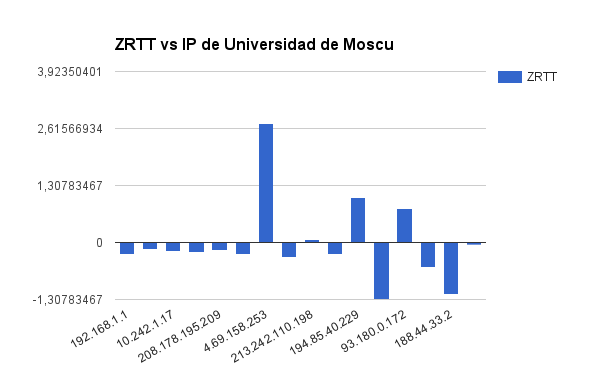
\includegraphics[width=\textwidth]{imgs/moscu.png}
\end{center}


\subsection{Universidad de Tokio}
Acontinuación mostramos los resultados obtenidos cuando tomamos como destino la
Universidad de Tokio (www.u-tokyo.ac.jp).

\begin{figure}[H]
\begin{center}
\begin{tabular}{|c|c|c|c|c|}
  \hline
  HOP & RTT & RTT RELATIVO & Ubicación & ZRTT \\ \hline
  192.168.1.1 & 62 ms & 0 & - & -0,3018867925 \\ \hline
  10.21.192.1 & 159 ms &  97  & - &  1,528301887 \\ \hline
  10.242.1.17 & 123 ms &  -36 & - & -0,9811320755 \\ \hline
  195.22.220.33 & 76 ms & -47 & (Italy) & -1,188679245 \\ \hline
  195.22.220.32 & 127 ms &  51  & (Italy)&  0,6603773585 \\ \hline
  195.22.219.145 &  160 ms &  33  & (Italy)&  0,320754717 \\ \hline
  195.22.219.145 &  95 ms & -65 & (Italy) & -1,528301887 \\ \hline
  149.3.181.65 &  106 ms &  11  & (Italy) & -0,09433962264 \\ \hline
  129.250.2.227 & 222 ms &  116 & Englewood (United States)&  1,886792453 \\ \hline
  129.250.4.13 &  272 ms &  50  & Englewood (United States)&  0,641509434 \\ \hline
  129.250.2.54 &  269 ms &  -3  & Englewood (United States) & -0,358490566 \\ \hline
  129.250.3.86 &  418 ms &  \textbf{149} & Englewood (United States)&  \textbf{2,509433962} \\ \hline
  129.250.6.188 & 405 ms &  -13 & Englewood (United States) & -0,5471698113 \\ \hline
  129.250.2.255 & 404 ms &  -1  & Englewood (United States) & -0,320754717 \\ \hline
  61.200.80.218 & 396 ms &  -8  & (Japan) & -0,4528301887 \\ \hline
  158.205.192.173 & 414 ms &  18  & (Japan)&  0,03773584906 \\ \hline
  158.205.192.86 &  413 ms &  -1  & (Japan) & -0,320754717 \\ \hline
  158.205.121.250 & 387 ms &  -26 & (Japan) & -0,7924528302 \\ \hline
  154.34.240.254 &  407 ms &  20  & (Japan)&  0,07547169811 \\ \hline
  210.152.135.178 & 399 ms &  -8  & (Japan) & -0,4528301887 \\ \hline
\end{tabular}
\caption{Tabla generada por Tracerout a la Universidad de Tokyo (210.152.135.178)}
% \label{my-label}
\end{center}
\end{figure}


\begin{center}
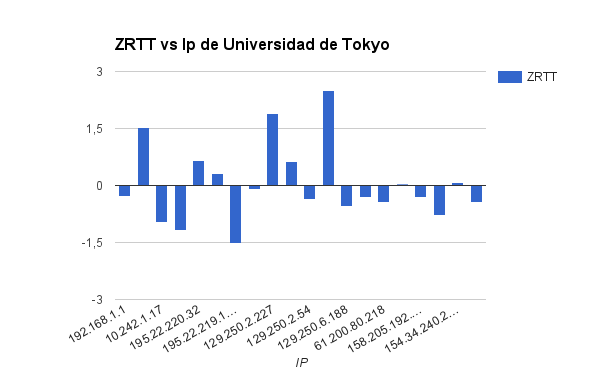
\includegraphics[width=\textwidth]{imgs/tokyo.png}
\end{center}


\subsection{Universidad de Sydney}
\begin{figure}[H]
\begin{center}
\begin{tabular}{|c|c|c|c|c|}
  \hline
  HOP & RTT & RTT RELATIVO & Ubicación & ZRTT \\ \hline
  192.168.1.1     & 83 ms  & 0          & - & -0,3940627873 \\ \hline
  10.21.192.1     & 167 ms & 84         & - & 0,7093130172  \\ \hline
  10.242.1.17     & 83 ms  & -84        & - & -1,497438592  \\ \hline
  195.22.220.33   & 67 ms  & -16        & - & -0,6042296073 \\ \hline
  195.22.220.32   & 78 ms  & 11         & - & -0,2495730986 \\ \hline
  195.22.206.190  & 270 ms & 192        & - & 2,127939052   \\ \hline
  198.32.176.177  & 312 ms & 42         & - & 0,1576251149  \\ \hline
  202.158.194.176 & 419 ms & 107        & - & 1,011427821   \\ \hline
  113.197.15.146  & 458 ms & 39         & - & 0,1182188362  \\ \hline
  138.44.5.47     & 416 ms & -42        & - & -0,9457506896 \\ \hline
  * * *           &        &            & - & -0,3940627873 \\ \hline
  * * *           &        &            & - & -0,3940627873 \\ \hline
  129.78.5.8      & 413 ms & -3         & - & -0,4334690661 \\ \hline
\end{tabular}
\caption{Tabla generada por Tracerout a la Universidad de Sydeny (129.78.5.8)}
% \label{my-label}
\end{center}
\end{figure}


\begin{center}
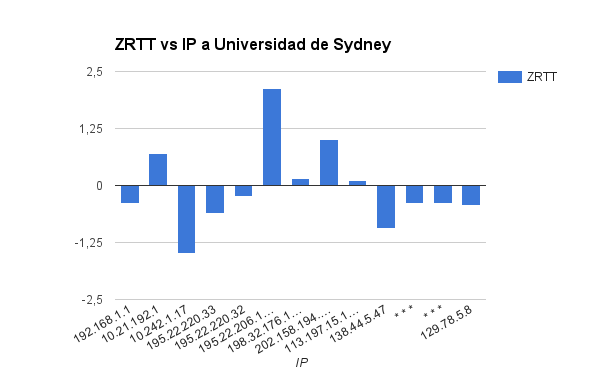
\includegraphics[width=\textwidth]{imgs/sydney.png}
\end{center}




